\documentclass[conference]{IEEEtran}
\usepackage{cite}
\usepackage{amsmath,amssymb}
\usepackage{graphicx}
\usepackage{booktabs}
\usepackage{array}
\usepackage{url}
\begin{document}
\title{Retrospective Daily Fire-Hotspot Occurrence Modelling in California\\Using ERA5, VIIRS, MODIS, and SRTM}
\author{\IEEEauthorblockN{Ayush Singh}\IEEEauthorblockA{Department of Computational Intelligence\\SRM Institute of Science and Technology\\Kattankulathur, India\\as5790@srmist.edu.in}
\and\IEEEauthorblockN{Sarvadnya Kulkarni}\IEEEauthorblockA{Department of Computational Intelligence\\SRM Institute of Science and Technology\\Kattankulathur, India\\ss9878@srmist.edu.in}}
\maketitle
\begin{abstract}
We evaluate daily satellite fire-hotspot occurrence on a $0.25^\circ$ California grid using observed ERA5 weather, VIIRS active-fire detections, MODIS vegetation composites, and SRTM terrain. A detection is a hotspot occurrence rather than a verified new ignition. The chronological split trains on 2021, selects the additive formulation on 2022, and evaluates the frozen fits on 2023. Of 240,029 test cell-days, 5,360 contain at least one qualifying VIIRS detection (2.23\%). The selected additive logistic model obtains test AUC-ROC 0.714, average precision 0.0682, and Brier score 0.02143. A same-cell hotspot-persistence baseline obtains AUC-ROC 0.762. The top decile of additive scores contains 27.1\% of test hotspots. These retrospective associations support a transparent comparison of weather, vegetation, terrain, and recent-fire features; same-day reanalysis inputs and active-fire labels do not establish prospective ignition forecasting skill.
\end{abstract}
\begin{IEEEkeywords}
Wildfire, active fire, hotspot occurrence, ERA5, VIIRS, MODIS, SRTM, calibration.
\end{IEEEkeywords}

\section{Introduction}
Fire activity depends on weather, fuel, terrain, and human sources of ignition. Satellite active-fire detections provide a spatially extensive observation of fire activity, but an active-fire pixel can persist across overpasses and days. The target in this paper is therefore whether a California grid cell contains a qualifying VIIRS hotspot on a given UTC day, not whether a new fire started there. This distinction is important when interpreting recent-fire predictors and high classification scores~\cite{schroeder}.

Physical ideas motivate interpretable predictors: heat and atmospheric dryness affect fuel conditions, vegetation indices approximate fuel availability and canopy water status, slope and wind can favour spread, and recent fire radiative power (FRP) measures prior observed activity~\cite{jones,wooster}. We compare a sign-constrained additive logistic model with an unconstrained fit, a multiplicative composite, tree ensembles, a simplified weather index, and strong seasonal and persistence baselines. The study asks how these retrospective formulations rank observed hotspot cell-days across an unseen year. It does not use forecast weather or infer causes of ignition.

\subsection{Research questions and contribution}
Three questions guide the comparison. First, do the proposed environmental formulations rank hotspot occurrence more effectively than recent hotspot history alone? Second, does imposing an expected positive direction on every transformed driver improve the ranking? Third, does a useful ranking also produce probabilities that improve on a constant event-rate forecast? These questions require different checks. Persistence addresses the first, the two additive fits inform the second, and calibration and Brier skill address the third. A single discrimination score cannot answer all three.

The contribution is an auditable comparison under a common observation target and chronological split. It includes negative findings: the selected additive formulation does not outperform persistence, its probability skill is modest, and the largest ablation loss does not identify a causal driver. The value of a transparent formula is that these failures can be examined explicitly. The experiment does not establish a new fire-danger law or a generally superior forecasting algorithm.

\section{Data and Study Design}
\subsection{Sources and spatial unit}
The study covers 1 January 2021 through 31 December 2023. ERA5 single-level hourly reanalysis supplies 2-m temperature, 2-m dewpoint, both 10-m wind components, and volumetric soil water in the 0--7 cm layer~\cite{era5}. Regional ERA5 tiles were read from the public Earthmover archive~\cite{earthmover}; a sampled grid-point hour in each of two months was compared with direct Copernicus downloads. NASA FIRMS standard-processing VIIRS S-NPP 375-m detections provide the response, FRP, and prior hotspot counts~\cite{firms,schroeder}. We retain presumed vegetation fires (type 0) at nominal or high confidence. NASA MOD13A2.061 supplies 1-km, 16-day NDVI and near/mid-infrared reflectances~\cite{modis}. SRTM elevation tiles yield static slope~\cite{srtm}. All raw sources and acquisition metadata are kept with the reproducible code package.

The working bounding box is $32$--$42^\circ$N and $124$--$114^\circ$W. We use only $0.25^\circ$ cell centres inside the US Census California boundary, giving 660 cells. A positive cell-day has at least one retained VIIRS detection. Multiple detections in the same cell-day count as one positive label. This is an observational detection target: cloud, smoke, overpass time, and sensor sensitivity can cause missed activity, while a continuing fire can contribute positives on successive days.

\subsection{Temporal alignment and feature construction}
ERA5 hours are aggregated by UTC day. We use maximum 2-m temperature, wind speed maximum, mean surface soil moisture, and relative humidity computed from temperature and dewpoint at the hour of the daily temperature maximum. The stored feature name \texttt{rh\_min} is a legacy name for this last quantity; it is not the minimum over all 24 hourly humidity estimates. MODIS NDWI is $(\mathrm{NIR}-\mathrm{MIR})/(\mathrm{NIR}+\mathrm{MIR})$. A 16-day composite is made available only after its full window and carried forward until the next available composite; no later composite is interpolated backward. SRTM pixel slopes are averaged within grid cells. Current-day FRP and counts are excluded from predictors; their histories use only days $t-1$ through $t-7$ with weight $0.5^k$ at lag $k$.

Each continuous driver is min--max scaled using only 2021 values, clipped to $[0,1]$ in later years, and then held fixed. Cells with missing MODIS indices are omitted. These rules prevent test-year information from entering the feature scaling or satellite composites. They do not make the study prospective because the same-day ERA5 aggregates are known only after the day.

\subsection{Observation support and missingness}
The spatial mask applies to grid-cell centres. Consequently, a retained coastal or border cell may include water or land outside the state; detections are assigned to the entire cell. The response should be interpreted at that spatial support. MODIS indices are nearest-neighbour samples at grid locations, whereas terrain slopes are cell means. These operations preserve different kinds of spatial variation. In particular, a sampled vegetation pixel need not represent every fuel type within a coarse cell.

Annual source-label totals and model-ready totals have different denominators. The source grid contains 5,376 positive cell-days in 2023, while complete model inputs retain 5,360. Metrics use only the latter rows. Omitting missing vegetation observations may change the evaluated population if missingness is associated with land cover or observation conditions. The current analysis does not estimate that selection effect. Likewise, delaying a composite by its window length prevents use of an unfinished window, but does not reproduce an operational product's actual publication latency.

\section{Models and Evaluation}
\subsection{Physically motivated formulations}
Let tildes denote training-scaled values. The nine additive inputs are $\tilde T$, $\widetilde{\mathrm{NDVI}}$, $1-\widetilde{\mathrm{NDWI}}$, $1-\widetilde{\mathrm{RH}}$, $1-\widetilde{\mathrm{SM}}$, $\tilde U$, $\tilde\theta$, $\widetilde{\mathrm{FRP}}_{\rm hist}$, and $\widetilde{\mathrm{Count}}_{\rm hist}$. The additive probability is
\begin{equation}
 p_t=\sigma\left(b+\sum_{j=1}^{9}w_jx_{jt}\right),\quad
 \sigma(z)=\frac{1}{1+e^{-z}}.
\end{equation}
The constrained version fits Bernoulli log loss with $w_j\geq0$, while the unconstrained version uses $L_2$-regularised logistic regression ($C=1$). The positive-coefficient restriction expresses the stated direction of each transformed feature; it is an assumption to test, not a physical law. Because the fits also differ in regularisation, their comparison does not isolate the effect of the sign restriction. Selection between the two uses only 2022 validation AUC-ROC. Dropping each variable involves a fresh fit of the same formulation on 2021.

For the multiplicative alternative we define
\begin{align}
 D_t &= a_1(1-\widetilde{\mathrm{NDWI}}_t)
       +a_2(1-\widetilde{\mathrm{RH}}_t)\notag\\
     &\quad +a_3(1-\widetilde{\mathrm{SM}}_t),\\
 H_t &= 0.6\widetilde{\mathrm{FRP}}_{{\rm hist},t}
       +0.4\widetilde{\mathrm{Count}}_{{\rm hist},t},\\
 R_t &= \tilde T_t\widetilde{\mathrm{NDVI}}_tD_t\notag\\
     &\quad\cdot(1+c_1\tilde U_t+c_2\tilde\theta_t)+H_t.
\end{align}
Six prespecified $(a_1,a_2,a_3,c_1,c_2)$ combinations are compared on 2022; a one-dimensional logistic mapping fitted on 2021 turns the selected index into probabilities. Factor ablations remove one factor and refit that mapping. This composite is a proposed index, not the Canadian Fire Weather Index (FWI).

\subsection{What the composite formula assumes}
The environmental part of $R_t$ is a product. It therefore approaches zero when any of its temperature, vegetation, or dryness factors approaches zero, even when the other factors are large. Adding $H_t$ allows recent fire activity to contribute independently of this gate. This is a substantive modelling choice: it imposes interactions before looking at the data, whereas the additive logit estimates separate linear contributions and the trees can represent conditional responses.

Training-scaled zero has no universal physical meaning. For temperature it denotes the minimum in the training population, not a combustion threshold. The product consequently depends on the chosen scaling origin as well as the five selected weights. Its bounded factors do not make the resulting score a probability; that interpretation comes only from the fitted logistic mapping. No mechanistic interpretation is attached to a fitted coefficient of that mapping.

Removing a multiplicative factor replaces it by one, except that removing recent activity sets its additive term to zero. Thus a factor ablation changes the structure of the index and refits its probability mapping. It differs from removing one variable from a multivariable logistic fit. Both analyses measure predictive sensitivity of a specified fitting procedure, rather than the effect of changing an environmental condition in the field.

\subsection{Comparators and metrics}
The remaining comparators are raw standardized nine-variable logistic regression; a training-cell rate with annual sine/cosine seasonality; same-cell previous-day and prior-week hotspot persistence; a temperature--dryness--wind index; and Random Forest, XGBoost, and LightGBM. Standardisation changes the effective $L_2$ penalty relative to the min--max-scaled additive fit. The trees use 200 estimators. Training-only SMOTE raises the minority/majority ratio to 0.10, followed by random undersampling to 0.30; the boosted trees additionally use class weights computed on this resampled set. Their scores receive a Platt logistic calibration on 2022; its validation Brier score is consequently in-sample. No test labels enter fitting, model choice, or calibration.

We report AUC-ROC, average precision (AP), and Brier score on validation and test years. AP should be compared with the observed positive-cell-day fraction. Brier skill is $1-B/B_{\rm train}$, where $B_{\rm train}$ is the 2023 Brier score of a constant probability equal to the 2021 event rate. The top-decile hit rate is the fraction of all 2023 hotspot cell-days inside the 10\% highest predicted probabilities. A paired day-block bootstrap samples 365 days with replacement 500 times; all positive rows and a fixed 5\% sample of negative rows enter this exploratory AUC comparison. Its interval applies to this sampled subset, not the full-test Brier score.

\section{Results}
\subsection{Observed prevalence and model performance}
The annual positive cell-day counts are 6,702 (2021), 4,889 (2022), and 5,376 (2023). The corresponding rates are 2.78\%, 2.03\%, and 2.23\%. Same-cell prior-day hotspot persistence is substantial: 33.4\% of test rows with a prior-day hotspot also have a current-day hotspot. This makes persistence an essential comparator.

The 2022-selected additive formulation is the unconstrained fit. Table~\ref{tab:results} gives all saved validation and test results. On 2023, it records AUC-ROC 0.714 and AP 0.0682 against an event-rate no-skill AP of 0.0223. The other additive formulation records AUC-ROC 0.711 and AP 0.1456, illustrating that selection by AUC alone need not select the best precision--recall ranking. The persistence comparator records AUC-ROC 0.762 and AP 0.1566. The highest test AUC in the table belongs to Random Forest (0.860; AP 0.2771). The simplified weather score is a three-variable reference, not an implementation of FWI. Figure~\ref{fig:discrimination} plots the held-out ROC and precision--recall curves from the same saved probabilities as Table~\ref{tab:results}.

\begin{table*}[!t]
\caption{2022 validation and 2023 test performance. AP denotes average precision.}
\label{tab:results}\centering\footnotesize\setlength{\tabcolsep}{3.7pt}
\begin{tabular}{lrrrrrr}\toprule
 & \multicolumn{3}{c}{2022 validation} & \multicolumn{3}{c}{2023 test}\\
Model & AUC & AP & Brier & AUC & AP & Brier\\\midrule
Constrained additive & 0.690 & 0.1038 & 0.01919 & 0.711 & 0.1456 & 0.02070 \\
\textbf{Unconstrained additive} & 0.711 & 0.0545 & 0.01968 & 0.714 & 0.0682 & 0.02143 \\
Raw standardized logistic & 0.756 & 0.1193 & 0.01895 & 0.758 & 0.1477 & 0.02052 \\
Cell and season climatology & 0.774 & 0.0793 & 0.02000 & 0.767 & 0.0774 & 0.02193 \\
Hotspot persistence & 0.758 & 0.1356 & 0.01820 & 0.762 & 0.1566 & 0.01942 \\
Multiplicative composite & 0.600 & 0.0295 & 0.02026 & 0.640 & 0.0357 & 0.02188 \\
Simplified weather index & 0.514 & 0.0198 & 0.02000 & 0.556 & 0.0236 & 0.02185 \\
Random Forest & 0.859 & 0.2386 & 0.01751 & 0.860 & 0.2771 & 0.01876 \\
XGBoost & 0.849 & 0.2231 & 0.01784 & 0.848 & 0.2526 & 0.01928 \\
LightGBM & 0.850 & 0.2299 & 0.01775 & 0.850 & 0.2577 & 0.01919 \\
\bottomrule\end{tabular}
\end{table*}

\begin{figure*}[!t]\centering
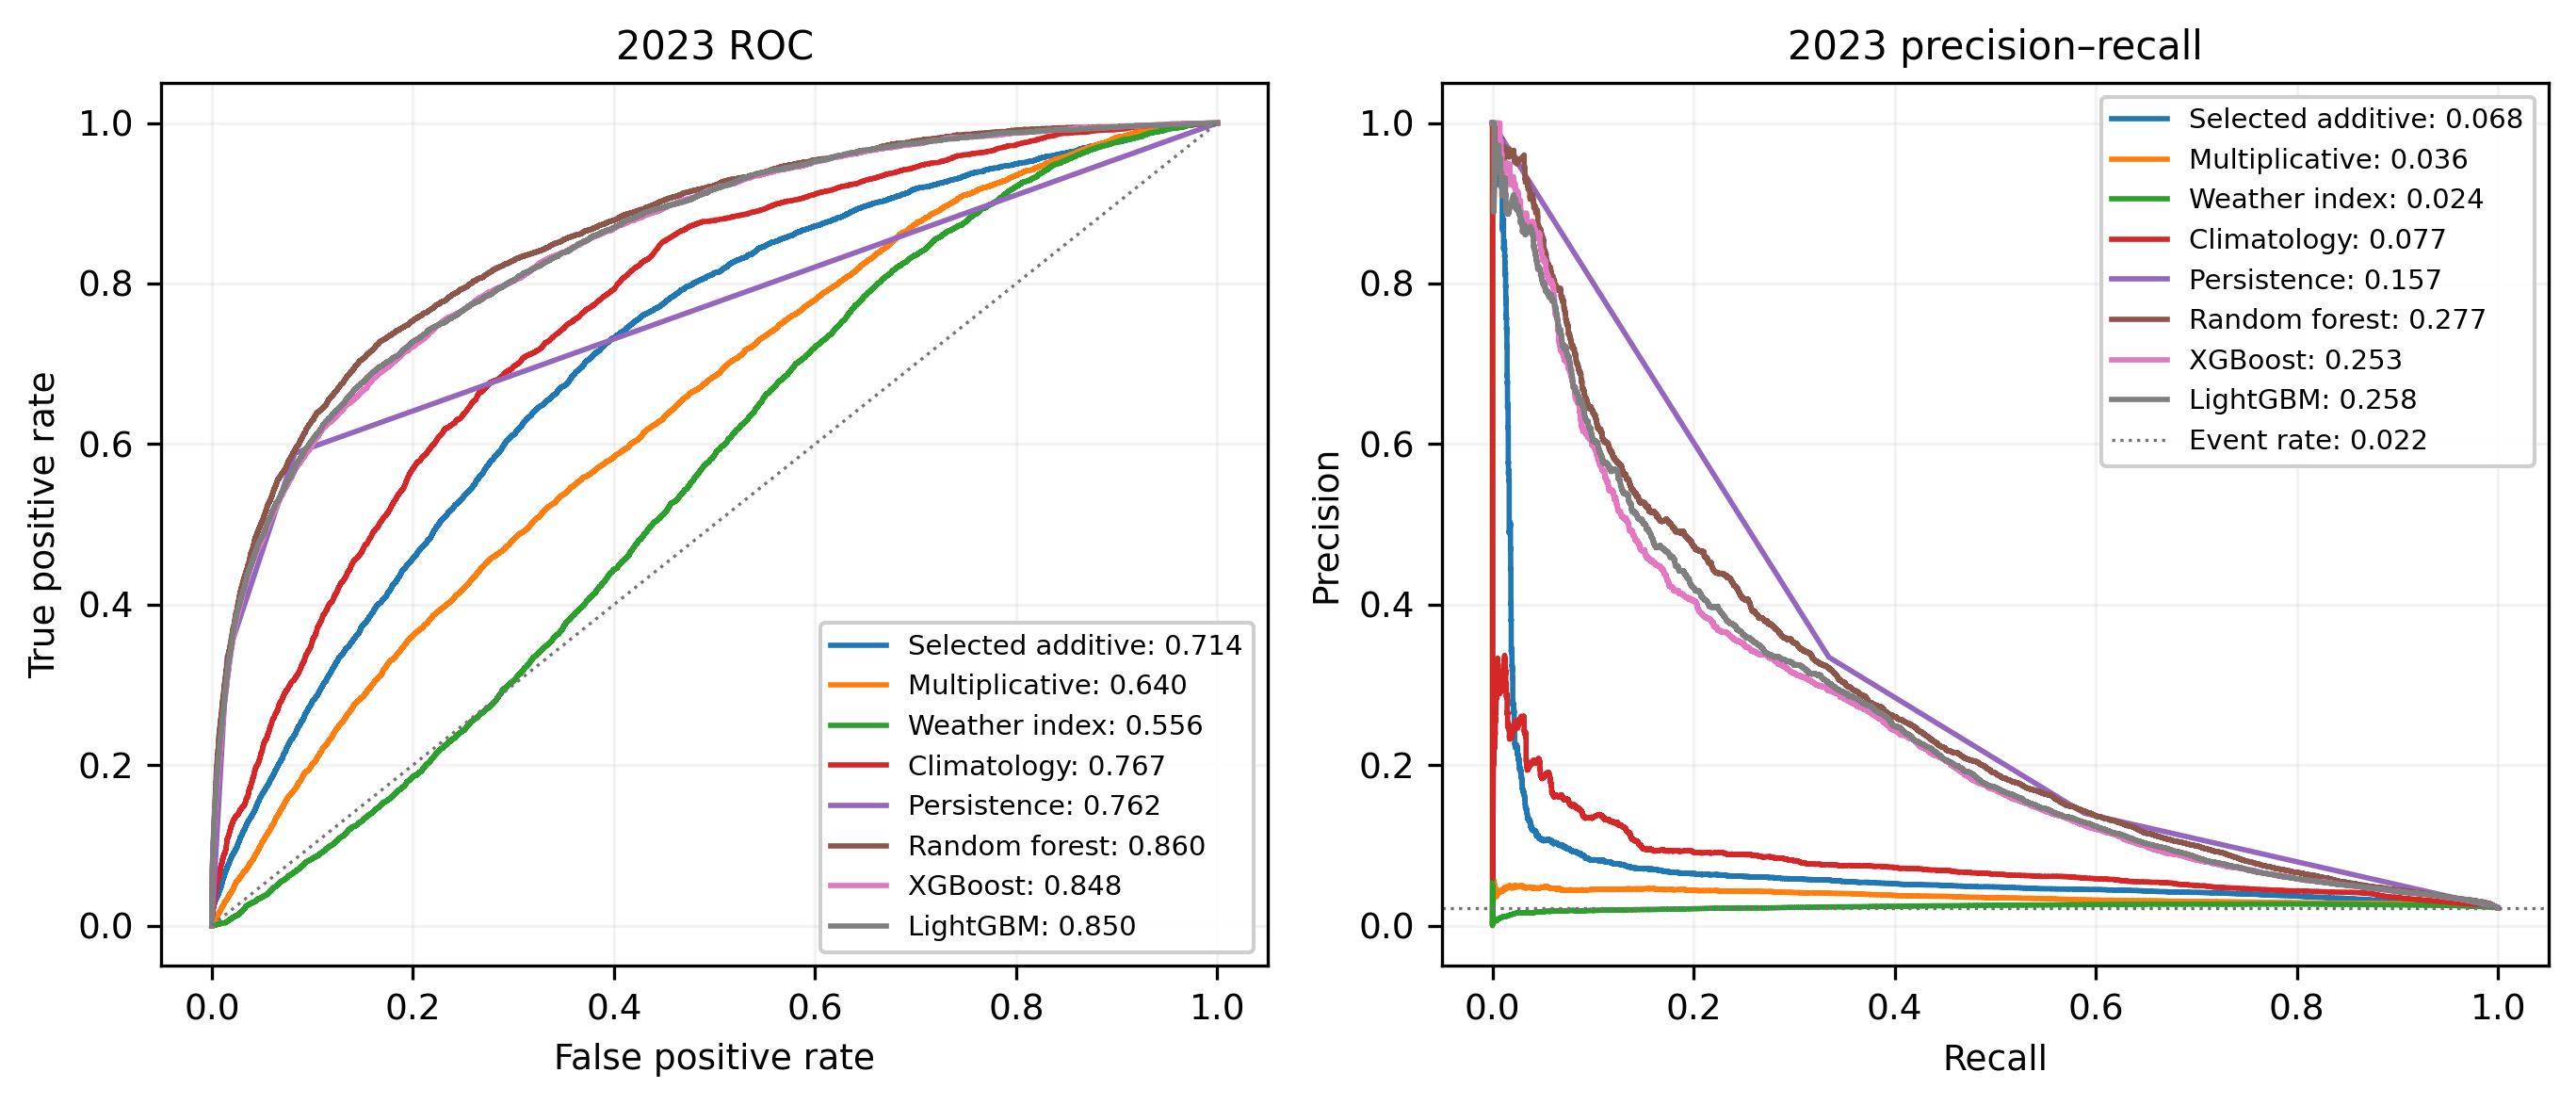
\includegraphics[width=.91\textwidth]{outputs/empirical_discrimination.png}
\caption{Held-out 2023 discrimination. Legends show AUC-ROC and average precision, respectively; the dotted precision--recall reference is the observed event rate.}
\label{fig:discrimination}\end{figure*}

\subsection{Coefficients and sensitivity}
Table~\ref{tab:coefs} lists the 2021 additive coefficients on min--max-scaled inputs and, separately, coefficients multiplied by each training standard deviation. Coefficients describe the fitted association conditional on the other inputs; correlated weather, vegetation, and history variables limit causal interpretation. The selected multiplicative weights are 0.30, 0.40, 0.30, 0.60, 0.40, giving validation AUC 0.600 and test AUC 0.640. The drop-one additive and factor-level multiplicative results appear in Figs.~\ref{fig:ablation_add} and~\ref{fig:ablation_mult}; the largest positive additive AUC loss is removing slope (drop 0.038). Removing a correlated feature may improve AUC because the model is refitted, so a negative loss is retained rather than hidden. The selected unconstrained fit assigns negative coefficients to 1-SM, U, slope; these conflict with the imposed directions in the constrained alternative and should not be read as physical effects.

\begin{table}[!t]\caption{Selected additive model: training-year coefficients.}\label{tab:coefs}
\centering\footnotesize\setlength{\tabcolsep}{4pt}
\begin{tabular}{lrr}\toprule
Input & Coefficient & Per training SD\\\midrule
$\tilde T$ & +1.123 & +0.188 \\
$\widetilde{\mathrm{NDVI}}$ & +5.960 & +1.128 \\
$1-\widetilde{\mathrm{NDWI}}$ & +3.775 & +0.625 \\
$1-\widetilde{\mathrm{RH}}$ & +1.632 & +0.363 \\
$1-\widetilde{\mathrm{SM}}$ & -1.515 & -0.413 \\
$\tilde U$ & -0.456 & -0.040 \\
$\tilde\theta$ & -1.880 & -0.423 \\
FRP history & +13.959 & +0.144 \\
Count history & +28.197 & +0.416 \\
Intercept & -8.647 & --- \\
\bottomrule\end{tabular}\end{table}

\begin{figure}[!t]\centering
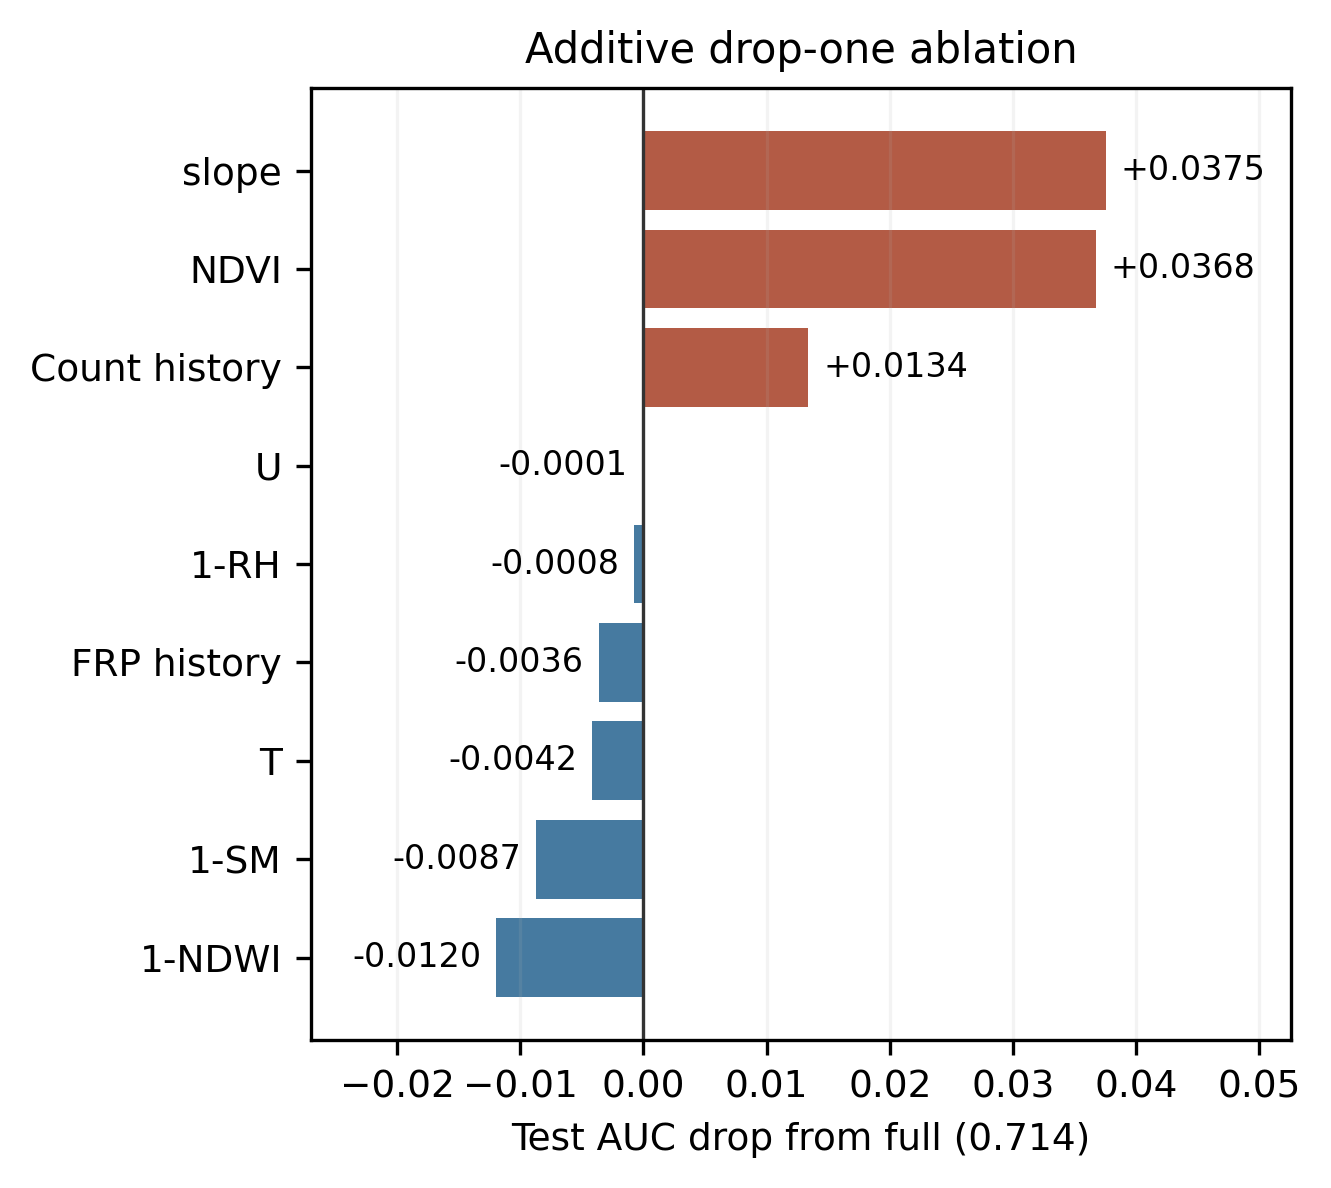
\includegraphics[width=.97\columnwidth]{outputs/empirical_additive_ablation.png}
\caption{2023 additive drop-one AUC change after refitting. Positive values favour the full model.}
\label{fig:ablation_add}\end{figure}
\begin{figure}[!t]\centering
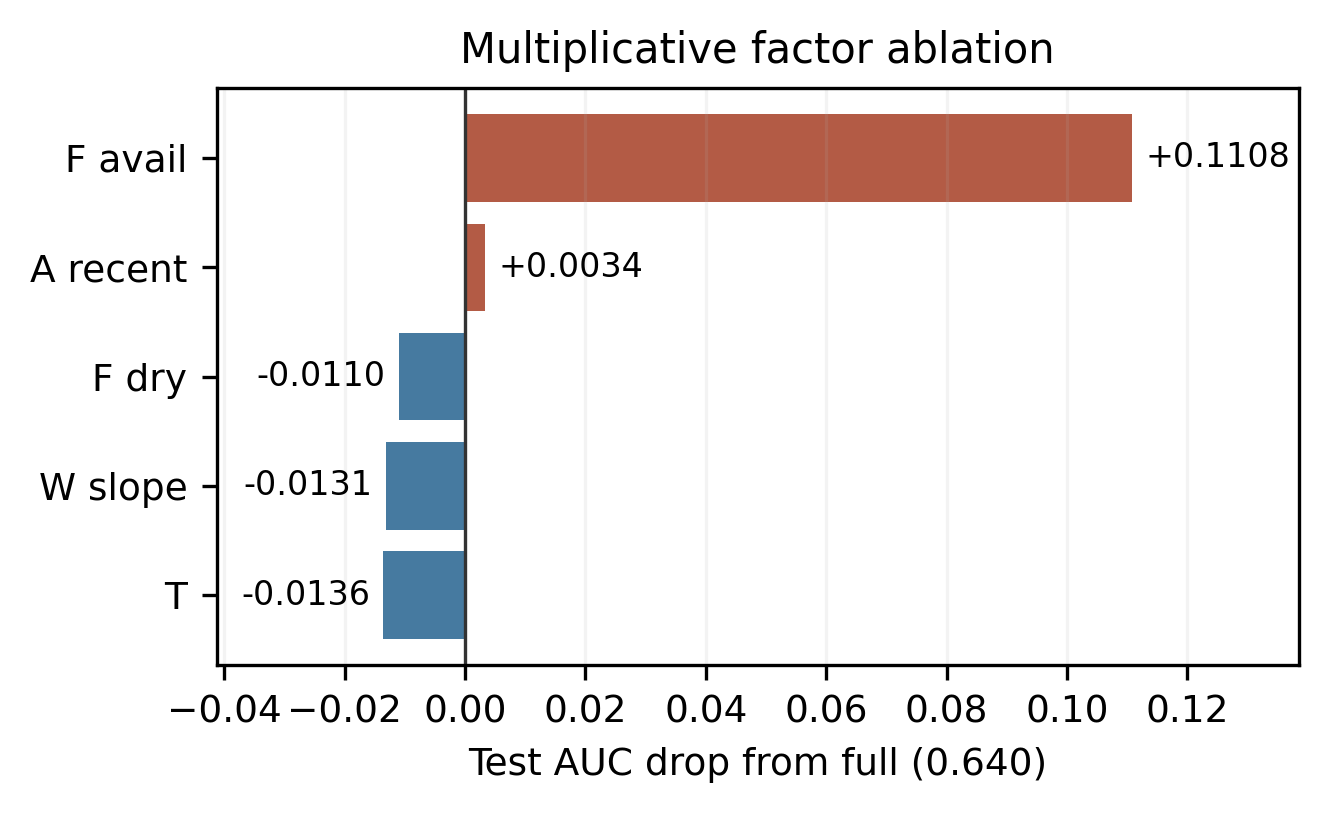
\includegraphics[width=.97\columnwidth]{outputs/empirical_multiplicative_ablation.png}
\caption{2023 multiplicative factor ablation. Positive values favour the full formulation.}
\label{fig:ablation_mult}\end{figure}

\subsection{Ranking and calibration}
The selected additive model has mean 2023 probability 0.0244 against an observed rate of 0.0223 (ratio 1.09). Its Brier score is 0.02143, versus 0.02186 for the constant 2021-rate forecast and 0.02183 for the constant 2023-rate reference; Brier skill relative to the training-rate reference is 0.0200. Figure~\ref{fig:reliability} groups the test predictions into equal-count bins. The largest absolute observed--predicted difference across the bins is 0.0133. The top decile threshold is 0.0536, selecting 10.0\% of rows and capturing 27.1\% of positives (lift 2.71 relative to random selection at the same fraction). These are retrospective ranks, not advance warnings.

\begin{figure}[!t]\centering
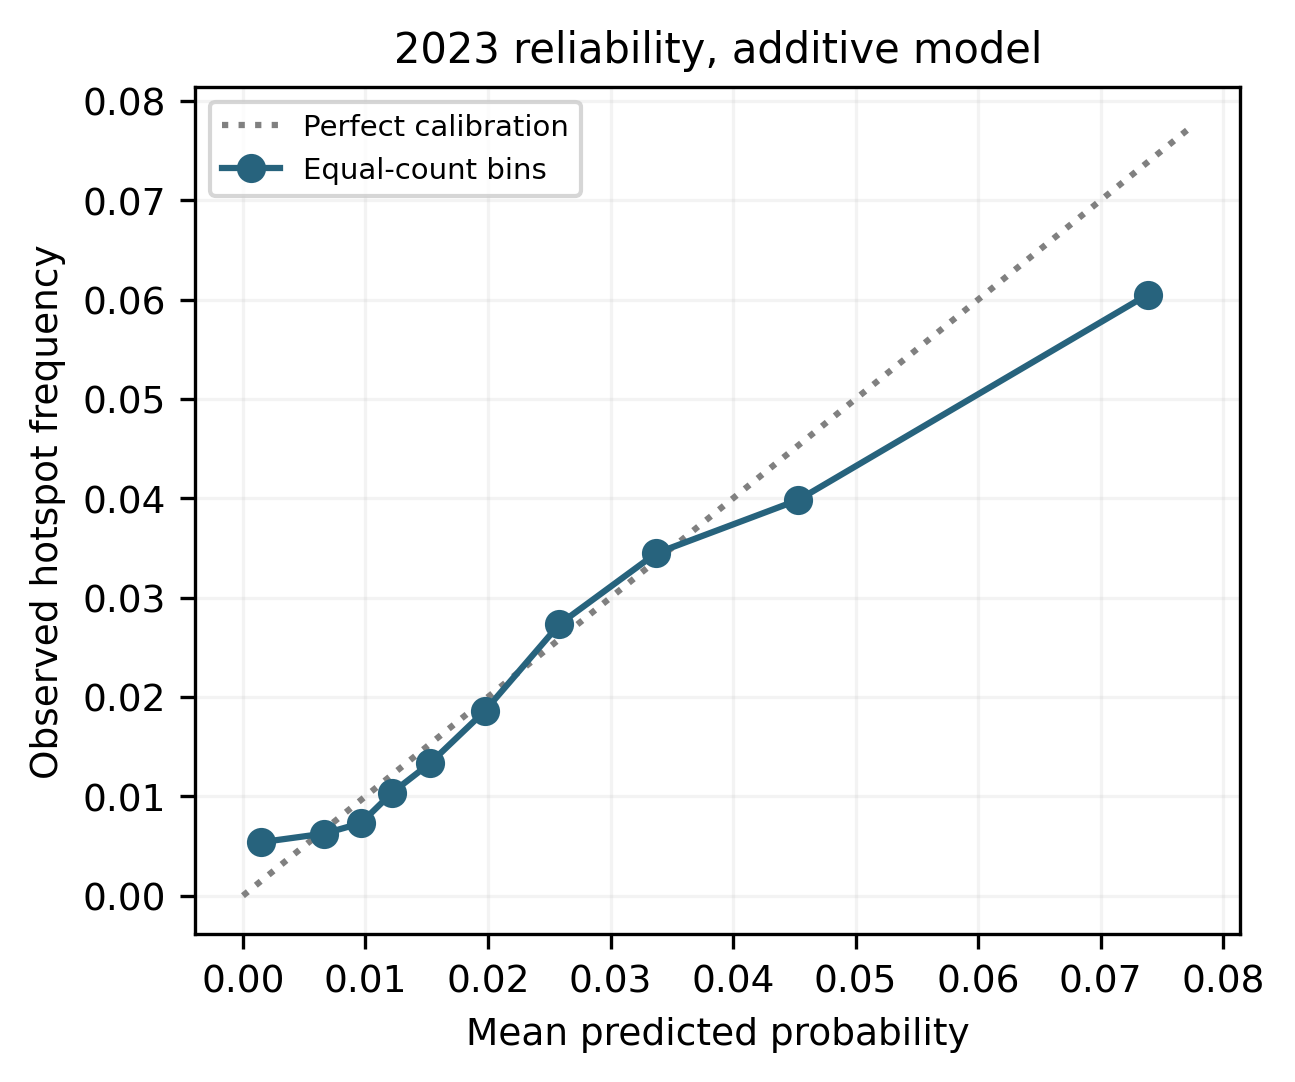
\includegraphics[width=.94\columnwidth]{outputs/empirical_reliability.png}
\caption{Observed 2023 hotspot frequency against mean selected-additive probability in equal-count prediction bins. The dotted line denotes exact calibration.}
\label{fig:reliability}\end{figure}

Figure~\ref{fig:shap} shows mean absolute SHAP values for a reproducible 3,000-row 2023 sample and the fitted XGBoost model. The largest value belongs to frp\_hist. SHAP magnitude describes that tree model's predictions; it neither establishes a physical cause nor transfers automatically to the additive model.
\begin{figure}[!t]\centering
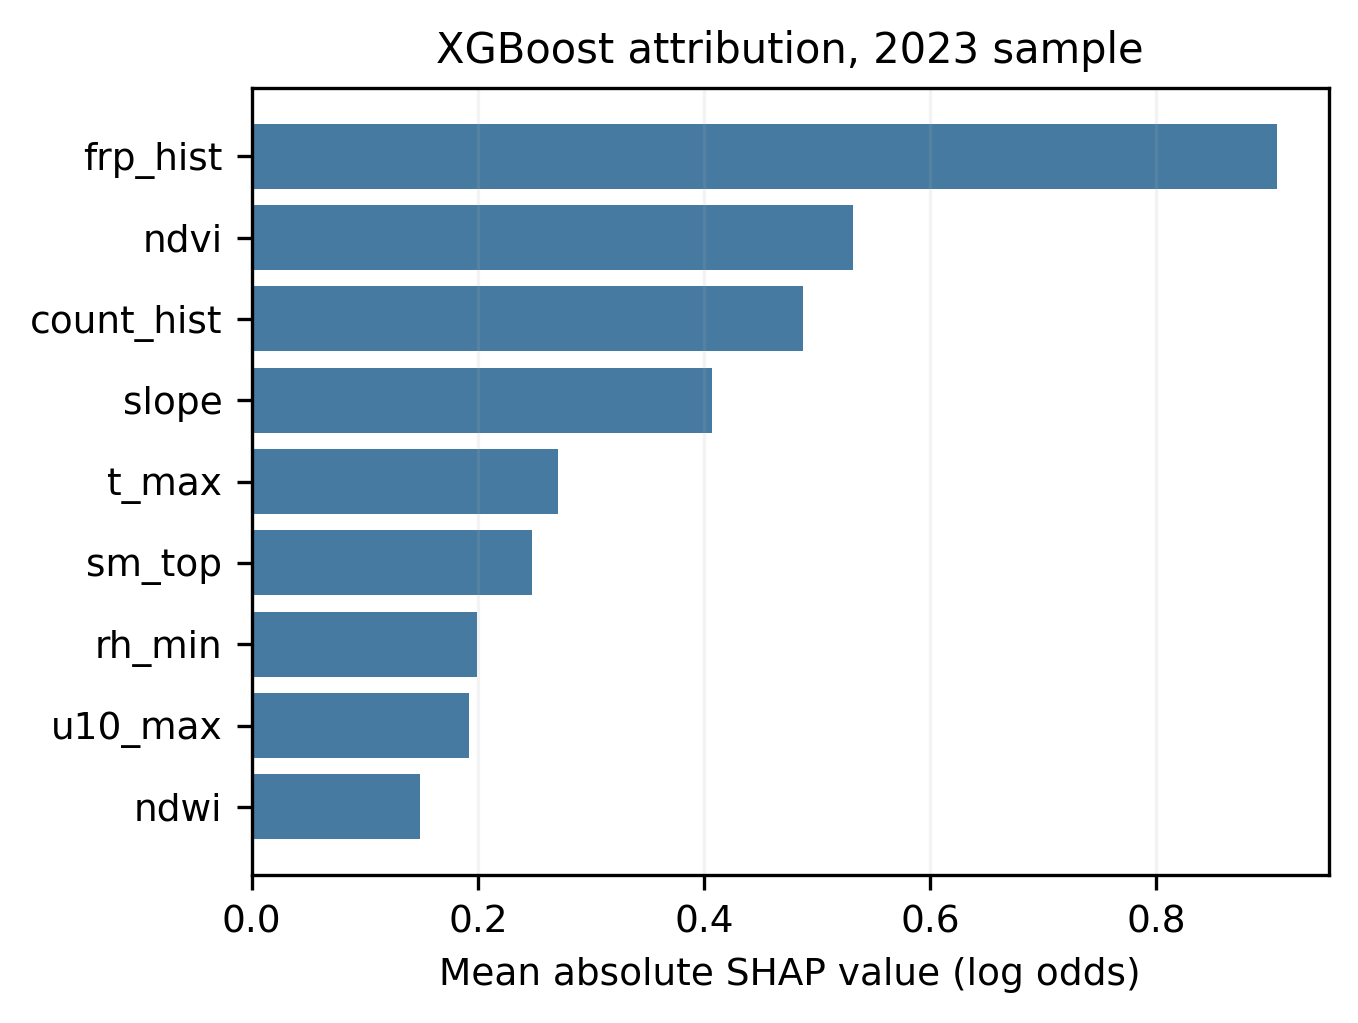
\includegraphics[width=.94\columnwidth]{outputs/empirical_shap.png}
\caption{Mean absolute SHAP attribution in the fitted XGBoost model on a fixed 2023 sample. Values are on the model's log-odds scale.}
\label{fig:shap}\end{figure}

\section{Discussion and Limitations}
\subsection{What the baseline comparisons establish}
The empirical comparison must be read alongside the simpler baselines. The selected additive model is 0.048 lower than persistence in AUC on the full 2023 test set. The weather-only logistic fit obtains AUC 0.569; adding surface soil moisture yields 0.591. These distinct fits do not form a nested sequence with the nine-variable drop-one ablation. The 2021-to-2023 change in event rate also affects probability calibration. Positive Brier skill is useful only to the extent shown by the actual reference score, and discrimination does not guarantee sharp or calibrated probabilities.

The same global top-decile threshold captures 40.5, 20.8, 15.1, 15.2\% of hotspots within the first through fourth slope quartiles, respectively. The corresponding NDVI-quartile capture fractions are 1.1, 4.2, 24.1, 48.7\%. These values are fractions of positives inside each quartile, not quartile-specific event rates. They show that the selected rank concentrates differently across terrain and vegetation strata; the observation does not isolate a causal slope or fuel effect. In the paired day-block bootstrap, the selected additive-minus-Random-Forest AUC difference has a 95\% interval of -0.157 to -0.137. That interval uses all sampled positive rows and a fixed 5\% sample of negative rows, so it is an exploratory comparison on an enriched subset.

The labels are active-fire detections, not confirmed new ignitions. Same-day ERA5 is retrospective, and lagged FRP/count features may reward monitoring of ongoing fires. A new-ignition or advance test needs incident-linked labels, forecast weather issued before the target day, and a lead-time split. MODIS cloud gaps and 16-day composites blur daily fuel detail; coarse cells mix land covers. One training and one test year do not establish transfer across regions or fire regimes. Prospective temporal and spatial validation is needed before operational use.

\subsection{Scaling, regularisation, and directional constraints}
The raw standardized logistic comparator reaches test AUC 0.758, compared with 0.714 for the selected min--max additive fit. These models use affine recodings of the same nine inputs. Without a penalty, an unconstrained linear logit can represent the same functions under either recoding, provided the transformations are invertible. With a fixed $L_2$ penalty, however, the cost assigned to a given change in a predictor's effect depends on its scale. The observed gap therefore cannot be credited to additional environmental information in the standardized model. It identifies scaling and regularisation as consequential parts of the fitting procedure.

The constrained fit also differs from the unconstrained fit in its penalty, so the present comparison cannot attribute their performance difference solely to signs. A matched comparison would use the same scaling and penalty strength, varying only the coefficient bounds. Penalty strength should be chosen within training data or a designated validation period. Since the 2023 outcomes have now been examined, selecting such a revision by its 2023 gain would turn this test year into development data. A later untouched year would be needed to evaluate the revised selection procedure.

The signs themselves require care. A negative slope coefficient is compatible with slope being useful for ranking; the ablation shows that removing slope harms this fitted model. Neither result implies that steep terrain prevents fire. Conditional coefficients can reflect geography, vegetation, human activity, observation support, and correlations with other predictors. Those mechanisms are not separated by this dataset. Similarly, adding soil moisture improves the restricted weather-only fit, while removing it improves the nine-variable fit. The two results concern different conditioning sets and different regularised optimisations.

\subsection{Ranking skill and the cost of an alert}
AUC averages ranking performance over thresholds that may be irrelevant to a practical monitoring budget. Here the constrained additive fit has lower AUC than the selected unconstrained fit, but substantially higher AP. This difference matters for a rare target: an analyst who can inspect only a small set of cells may prefer a different model from one selected by global AUC. The present selection criterion is retained so that the reported primary model follows the stated protocol. A future application should specify the monitoring budget and error costs before choosing its selection metric.

For the selected model, allocating attention to roughly 24,003 cell-days captures 1,452 of the 5,360 positives. Its precision at this budget is therefore about 6.05\%, while 72.9\% of positives fall outside the selected set. The 2.71-fold lift is useful evidence of concentration, but does not imply that most flagged cells contain a detected hotspot. These counts refer to cell-days and may include repeated observations of the same ongoing fire. They cannot be converted into numbers of distinct incidents or successful interventions.

The reliability diagram also supports a narrower conclusion than average calibration alone. In its highest equal-count bin, mean prediction is about 7.38\% and observed occurrence is 6.05\%; in its lowest bin the corresponding values are about 0.15\% and 0.54\%. Overprediction is therefore not uniform across the score range. A change in overall event rate may contribute to calibration drift, but does not by itself establish the cause of these conditional errors. With Brier skill of about 2\%, the selected model improves only modestly on the constant training-rate forecast despite its above-chance discrimination.

\subsection{Dependence and the next empirical test}
The bootstrap retains within-day spatial co-occurrence, but sampling individual days does not preserve dependence across adjacent days of a long-lived fire. Its intervals may therefore understate uncertainty from persistent episodes. Negative-row subsampling introduces another distinction between the bootstrap population and the complete test set. These intervals are useful sensitivity summaries, not evidence of transfer to a new region or a different fire regime. A longer time series would permit resampling multi-day blocks and evaluating several held-out years.

The strongest immediate research extension is to separate continued activity from newly detected activity. That would require an explicit event definition, such as incident linkage or a prespecified absence window, followed by checks for missed detections. Removing recent-fire predictors alone would not solve the label problem. For advance prediction, weather inputs must additionally be available at the forecast issue time. Both changes alter the scientific target and require a new evaluation, rather than a reinterpretation of the current scores.

A second extension is an ablation of the training procedure itself: compare class resampling with no resampling, match regularisation across additive variants, and fit calibration on a separate chronological segment. This would help identify whether gains arise from feature relationships, class handling, or calibration. None of those unperformed comparisons is claimed as a result here. The existing experiment instead establishes a reproducible starting point and shows which apparent physical assumptions fail to secure an advantage over simple history-based prediction.

\section{Conclusion}
Using newly acquired observed-source inputs, this study provides a reproducible California grid-cell comparison of physically motivated daily hotspot-occurrence models and strong nonphysical baselines. The validation-selected additive model scores 0.714 AUC-ROC and 0.0682 AP on 2023, while persistence scores 0.762 AUC-ROC. The supplied data, code, predictions, and figures permit direct checking of these claims. The result is a retrospective analysis of active-fire detections; it should not be described as verified ignition forecasting.

\section*{Acknowledgment}
The authors acknowledge the Copernicus Climate Data Store, NASA FIRMS and LP DAAC, the USGS, and the US Census Bureau for the source products used here.

\begin{thebibliography}{00}
\bibitem{schroeder} W.~Schroeder, P.~Oliva, L.~Giglio, and I.~A.~Csiszar, ``The new VIIRS 375 m active fire detection data product,'' \emph{Remote Sensing of Environment}, vol.~143, pp.~85--96, 2014, doi:10.1016/j.rse.2013.12.008.
\bibitem{jones} M.~W.~Jones \emph{et al.}, ``State of wildfires 2023--2024,'' \emph{Earth System Science Data}, vol.~16, pp.~3601--3685, 2024, doi:10.5194/essd-16-3601-2024.
\bibitem{wooster} M.~J.~Wooster, G.~Roberts, G.~L.~W.~Perry, and Y.~J.~Kaufman, ``Retrieval of biomass combustion rates and totals from fire radiative power observations,'' \emph{Journal of Geophysical Research: Atmospheres}, vol.~110, D24311, 2005, doi:10.1029/2005JD006318.
\bibitem{era5} Copernicus Climate Change Service, ``ERA5 hourly data on single levels from 1940 to present,'' Climate Data Store, doi:10.24381/cds.adbb2d47.
\bibitem{earthmover} Earthmover, ``Icechunk ERA5: public analysis-ready reanalysis archive,'' Registry of Open Data on AWS, \url{https://registry.opendata.aws/earthmover-era5/}, accessed Nov.~2026.
\bibitem{firms} NASA FIRMS, ``VIIRS S-NPP 375 m active fire detections: Standard Processing,'' \url{https://firms.modaps.eosdis.nasa.gov/content/descriptions/FIRMS_VIIRS_Firehotspots.html}, accessed Nov.~2026.
\bibitem{modis} NASA LP DAAC, ``MOD13A2.061 MODIS/Terra Vegetation Indices 16-Day L3 Global 1 km,'' \url{https://lpdaac.usgs.gov/products/mod13a2v061/}, accessed Nov.~2026.
\bibitem{srtm} NASA LP DAAC, ``SRTM Collection User Guide,'' \url{https://lpdaac.usgs.gov/documents/179/SRTM_User_Guide_V3.pdf}, accessed Nov.~2026.
\end{thebibliography}
\end{document}